\subsection{Cronograma}

El cronograma de actividades se estructura en seis fases principales que abarcan todo el período del 23 de febrero al 11 de julio de 2026. A continuación se describe cada actividad:

\begin{enumerate}
    \item \textbf{Presentación del perfil del proyecto (23 de febrero - 25 de marzo):} Elaboración y presentación del perfil del proyecto, incluyendo la definición del tema, establecimiento de objetivos, análisis de necesidades del mercado, definición de la localización del proyecto y elaboración del anteproyecto para su aprobación.

    \item \textbf{Realización del estudio de mercado (26 de marzo - 29 de abril):} Investigación de campo para recopilar información sobre el mercado objetivo, análisis de la competencia, definición de la demanda potencial y validación de la viabilidad del servicio de mensajería automatizada.

    \item \textbf{Análisis de ingeniería, tamaño, localización y administración (30 de abril - 3 de junio):} Diseño de la arquitectura de la plataforma, definición de módulos del sistema, diseño de agentes de autorrespuesta, definición de la organización del sistema y análisis de tamaño y capacidad del proyecto.

    \item \textbf{Evaluación de inversión, financiamiento, ingresos, costos y evaluación económica (4 de junio - 17 de junio):} Determinación de la inversión requerida, análisis de financiamiento, estimación de ingresos y costos operativos, y evaluación económica mediante indicadores de viabilidad.

    \item \textbf{Preparación de la presentación final (18 de junio - 24 de junio):} Elaboración de la documentación final del proyecto, incluyendo marco teórico, antecedentes, bases metodológicas, resultados y conclusiones.

    \item \textbf{Preparación de defensa final (25 de junio - 6 de julio):} Repaso general del proyecto, preparación de materiales para la defensa y ajustes finales antes de la presentación formal.

    \item \textbf{Entrega del producto (11 de julio):} Presentación y defensa oficial del proyecto final.
\end{enumerate}

\begin{center}
    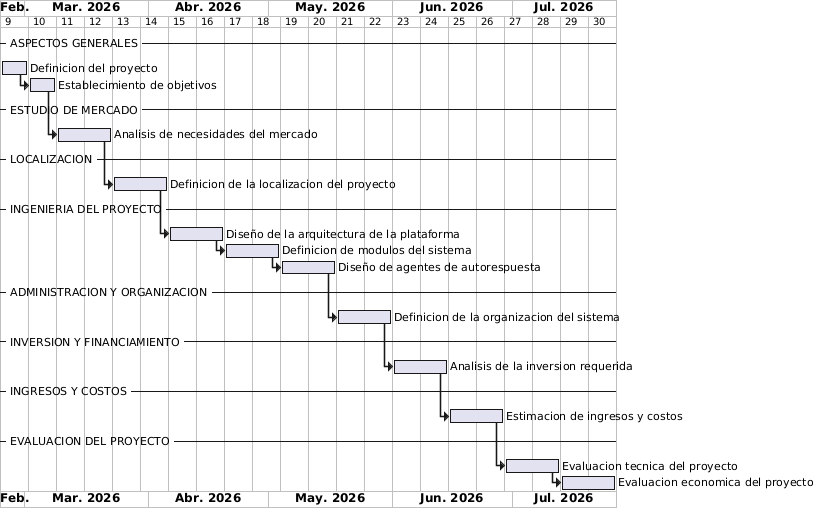
\includegraphics[width=\textwidth]{img/cronograma.png}
    \captionsetup{hypcap=false}
    \captionof{figure}{Cronograma de actividades del proyecto}
    \label{fig:cronograma}
\end{center}